\section{Computational models}


This section introduces some of the most important computational models in the history of computer science and explains \textit{why it doesn't matter.}



Uncomputability has an intimate connection to G\"{o}del's famous Incompleteness Theorem.



%%=============================================================================
\subsection{Turing machines}


% figure
\begin{figure}[h]
    \centering
    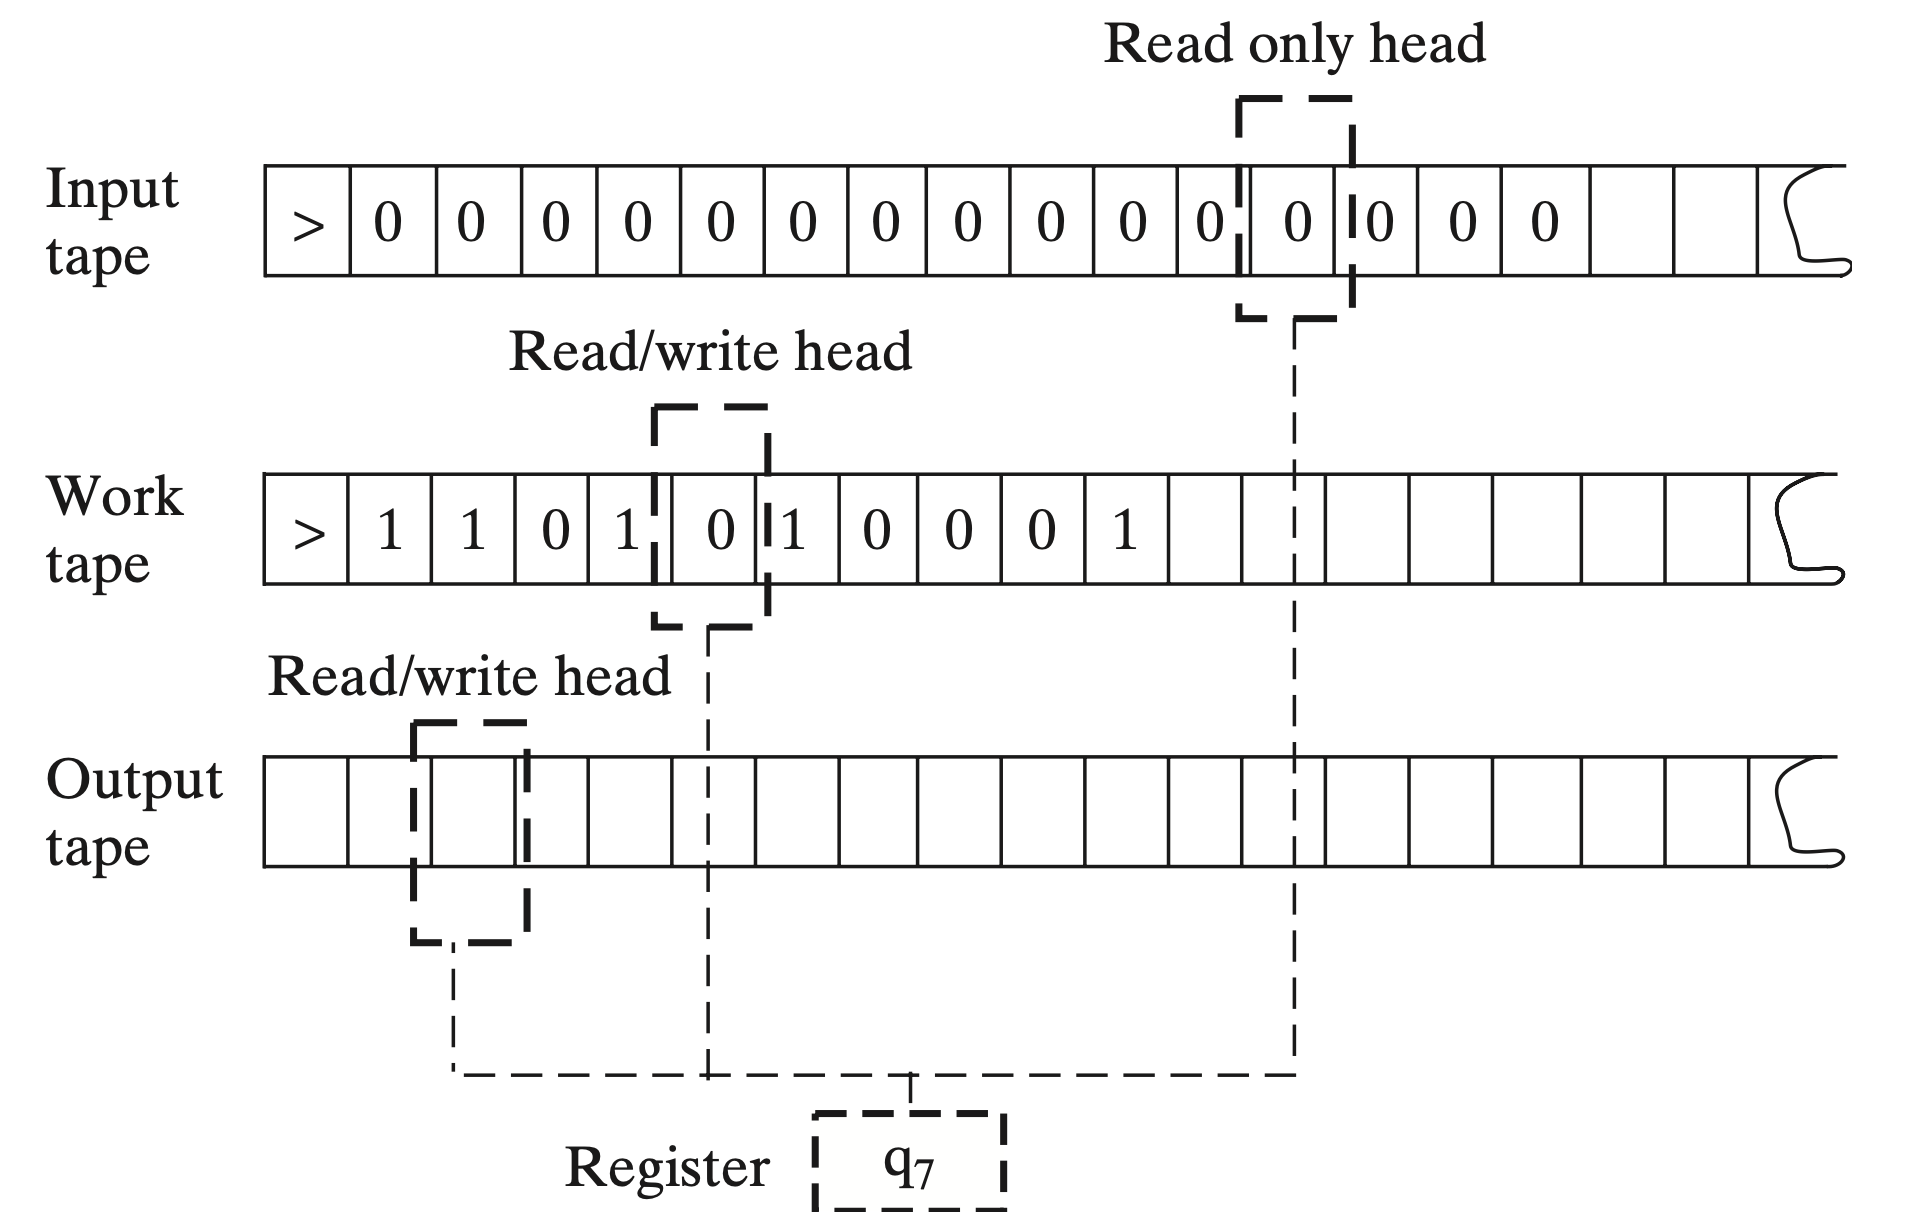
\includegraphics[width=.9\textwidth]{fig/three-tape-TM}
    \caption{A snapshot of the execution of a three--tape Turing machine M with an input tape, a work tape, and an output tape, see \cite[p.~11]{Aro.Bar2009}}
    \label{fig: three-tape-TM}
\end{figure}




A \textit{tape} is an infinite one--directional line of cells, each of which can store a symbol from a finite  set called \textit{alphabet}.
% 
Each tape is equipped with a \textit{tape head} that can potentially read or write symbols to the tape one cell at a time.



alphabet $\{0,1\} \cup \{\blank, \triangleright, \}$



state set $Q$, contains two distinguished states: 
the start state $q_{start}$ and the halting state $q_{halt}$







\begin{example}[palindrome \zh{回文}]
    A \textit{palindrome} is a string that reads the same forwards and backwards. 
    % 
    The language of palindromes over the binary alphabet is 
    \[
        PAL = \{ w \in \{0,1\}^* \mid w = w^R \}
    \]
    where $w^R$ denotes the reverse of $w$.
    % 
    For example, 
    $00100$ is a palindrome,
    and clearly $\{\epsilon,0,1\} \subseteq PAL$.
    % 
    
    A Turing machine that computes $PAL$ within less than $3|x|$ steps for any input $x$.

    Our TM $M$ will use three tapes (the input, work and output tape) and the alphabet $\{\blank,\triangleright,0,1\}$: 
    
    \vspace{1em}
    \begin{algorithmic}[1]
        \State Input $x$  (where $|x|=n$)

        \State 
        Copy $x$ to the work tape \qquad ($n$ steps)

        \State 
        Move the input--tape head the begining of $x$ \qquad ($n$ steps)

        \State 
        Move the input-tape head to the right while moving the work-tape head to the left.

        \If{at any moment the machine observes two different symbols}
            \State \textbf{reject} and output $0$
        \Else 
            \State \textbf{accept} and output $1$
        \EndIf  \qquad ($\leq n$ steps)
        \end{algorithmic}
\end{example}




%%=============================================================================
\subsection{Running Time}

Any nontrivial computational task requires at least reading the entire input, 
we count the number of basic steps as a function of the input length.



\begin{df}[Computing a function and running time]
    Given $f \colon \{0,1\}^* \to \{0,1\}^*$, 
    $T \colon \mathbb{N} \to \mathbb{N}$ and a Turing machine $M$, we say that
    % 
    \begin{enumerate}[itemsep=5pt,parsep=5pt,leftmargin=3em,topsep=5pt,label=(\arabic*)] %% or label = \alph*, \roman*
        \item $M$ \textit{computes} $f$ if for every $x \in \{0,1\}^*$, 
        whenever $M$ is initialized to the start configuration on input $x$, 
        then it halts with $f(x)$ on the output tape.

        \item 
        \textit{$M$ computes $f$ in $T(n)$--time} if its computation on every input $x$ requires at most $T(|x|)$ steps.
    \end{enumerate}
\end{df}




%%=============================================================================
\subsection{Machines as Strings and the Universal Turing Machine}

It is almost obvious that \textit{we can represent a Turing machine as a string}: 
Just write the description of the TM on paper, 
and encode this description as a sequence of zeros and ones.
% 
This string can be given as input to another Turing machine.






%%=============================================================================
\subsection{Variants of Turing machines}

\subsubsection{Turing machines with alphabet $\{0,1,\blank,\triangleright\}$}

\subsubsection{Single tape Turing machines}

\subsubsection{Bidirectional single tape Turing machines}







%%=============================================================================
\subsection{Other  computational models*}



%%-------------------------------------
\subsubsection{URM: the unlimited register machine}


